\documentclass[aspectratio=169,10pt]{beamer}

\usepackage[utf8]{inputenc}
\usepackage[T1]{fontenc}
\usepackage{amsmath,amssymb,amsthm}
\usepackage{graphicx}
\usepackage{listings}
\usepackage{xcolor}
\usepackage{tikz}
\usepackage{algorithm}
\usepackage{algorithmic}
\usepackage{hyperref}
\usepackage{mimic}

\usetheme{Madrid}
\usecolortheme{seahorse}
\setbeamertemplate{navigation symbols}{}
\setbeamertemplate{footline}[frame number]

\lstset{
    language=Python,
    basicstyle=\ttfamily\scriptsize,
    keywordstyle=\color{blue}\bfseries,
    stringstyle=\color{red},
    commentstyle=\color{green!60!black},
    showstringspaces=false,
    breaklines=true,
    breakatwhitespace=true,
    frame=single,
    numbers=left,
    numberstyle=\tiny\color{gray},
    xleftmargin=1em,
    framexleftmargin=1em
}

% Title page information
\title{Reinforcement Learning}
\subtitle{Lecture 11: Modern Directions \& Capstone: RLHF, DPO, MCTS, and AlphaZero}
\author{Taehoon Kim}
\institute{Sogang University MIMIC Lab \\ \url{https://mimic-lab.com}}
\date{Fall Semester 2025}

\begin{document}

% Slide 1: Title
\begin{frame}
  \titlepage
\end{frame}

% Slide 2: Today's Agenda
\begin{frame}{Today's Agenda}
  \begin{block}{Session Structure}
    \begin{itemize}
      \item \textbf{Theory Focus:} RLHF pipeline, DPO objectives, MCTS foundations, AlphaZero strategy
      \item \textbf{Practice Focus:} Implementation walkthroughs, experiment deep dives, project planning
    \end{itemize}
  \end{block}

  \begin{columns}[t]
    \begin{column}{0.5\textwidth}
      \textbf{Segment Highlights:}
      \begin{itemize}
        \item Course integration and roadmap
        \item RLHF theory and data pipelines
        \item Direct Preference Optimization techniques
      \end{itemize}
    \end{column}
    \begin{column}{0.5\textwidth}
      \textbf{Hands-on Emphasis:}
      \begin{itemize}
        \item MCTS rollouts with PUCT
        \item AlphaZero-style self-play implementation
        \item RLHF training utilities and evaluation
      \end{itemize}
    \end{column}
  \end{columns}
\end{frame}

% Slide 3: Learning Objectives
\begin{frame}{Learning Objectives \& Prerequisites}
  \begin{block}{By the end of this lecture, you will be able to:}
    \begin{itemize}
      \item Understand RLHF pipeline and regularized policy optimization
      \item Implement Direct Preference Optimization (DPO) without reward models
      \item Build MCTS with neural network guidance (PUCT algorithm)
      \item Create AlphaZero self-play training loops
      \item Design integrated capstone projects combining modern RL methods
    \end{itemize}
  \end{block}
  
  \begin{block}{Prerequisites}
    \begin{itemize}
      \item Policy gradient methods (Lectures 8-10)
      \item Neural network training and PyTorch proficiency
      \item Understanding of tree search algorithms
      \item Familiarity with preference learning concepts
    \end{itemize}
  \end{block}
\end{frame}


% Slide 5: RLHF Introduction
\begin{frame}{Reinforcement Learning from Human Feedback (RLHF)}
  \begin{block}{The Challenge}
    How do we train RL agents to follow human preferences when reward functions are hard to specify?
  \end{block}
  
  \begin{columns}[t]
    \begin{column}{0.5\textwidth}
      \textbf{Traditional RL:}
      \begin{itemize}
        \item Hand-crafted reward functions
        \item Often misaligned with human intent
        \item Reward hacking problems
        \item Difficult to specify for complex tasks
      \end{itemize}
    \end{column}
    \begin{column}{0.5\textwidth}
      \textbf{RLHF Approach:}
      \begin{itemize}
        \item Learn rewards from human preferences
        \item Three-stage pipeline: SFT $\rightarrow$ RM $\rightarrow$ RL
        \item Regularized policy optimization
        \item Scalable to complex domains
      \end{itemize}
    \end{column}
  \end{columns}
  
  \begin{alertblock}{Key Insight}
    Instead of engineering rewards, learn them from pairwise human comparisons of agent behaviors
  \end{alertblock}
\end{frame}

% Slide 6: RLHF Three-Stage Pipeline
\begin{frame}{RLHF Three-Stage Pipeline}
\begin{center}
    
  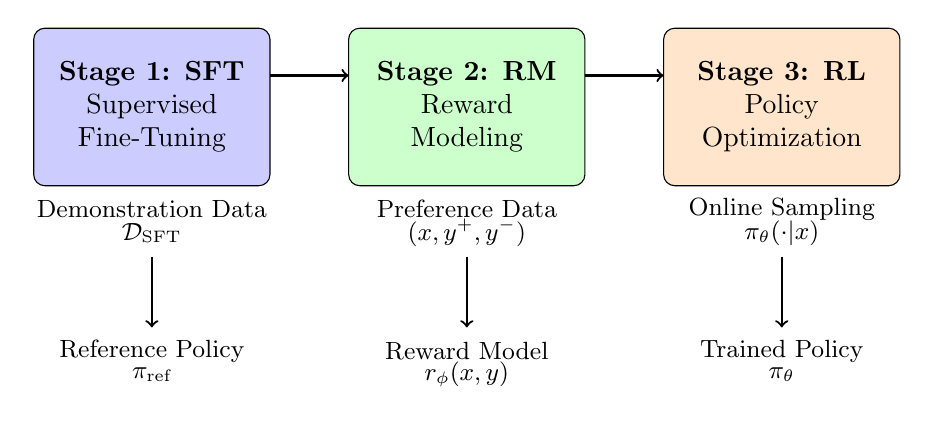
\begin{tikzpicture}[scale=1.0, transform shape]
    % Stage 1: SFT
    \node[draw, rounded corners, fill=blue!20, minimum width=3cm, minimum height=2.0cm, yshift=-0.4cm] at (2, 6) {
      \begin{minipage}{2.5cm}
        \centering
        \textbf{Stage 1: SFT} \\
        Supervised \\
        Fine-Tuning
      \end{minipage}
    };
    
    % Stage 2: RM
    \node[draw, rounded corners, fill=green!20, minimum width=3cm, minimum height=2.0cm, yshift=-0.4cm] at (6, 6) {
      \begin{minipage}{2.5cm}
        \centering
        \textbf{Stage 2: RM} \\
        Reward \\
        Modeling
      \end{minipage}
    };
    
    % Stage 3: RL
    \node[draw, rounded corners, fill=orange!20, minimum width=3cm, minimum height=2.0cm, yshift=-0.4cm] at (10, 6) {
      \begin{minipage}{2.5cm}
        \centering
        \textbf{Stage 3: RL} \\
        Policy \\
        Optimization
      \end{minipage}
    };
    
    % Data flows
    \node[anchor=center] at (2, 4.3) {\small Demonstration Data};
    \node[anchor=center] at (2, 4.0) {\small $\mathcal{D}_{\text{SFT}}$};
    
    \node[anchor=center] at (6, 4.3) {\small Preference Data};
    \node[anchor=center] at (6, 4.0) {\small $(x, y^+, y^-)$};
    
    \node[anchor=center] at (10, 4.3) {\small Online Sampling};
    \node[anchor=center] at (10, 4.0) {\small $\pi_\theta(\cdot|x)$};
    
    % Outputs
    \node[anchor=center] at (2, 2.5) {\small Reference Policy};
    \node[anchor=center] at (2, 2.2) {\small $\pi_{\text{ref}}$};
    
    \node[anchor=center] at (6, 2.5) {\small Reward Model};
    \node[anchor=center] at (6, 2.2) {\small $r_\phi(x, y)$};
    
    \node[anchor=center] at (10, 2.5) {\small Trained Policy};
    \node[anchor=center] at (10, 2.2) {\small $\pi_\theta$};
    
    % Arrows
    \draw[->, thick] (3.5, 6) -- (4.5, 6);
    \draw[->, thick] (7.5, 6) -- (8.5, 6);
    \draw[->, thick] (2, 3.7) -- (2, 2.8);
    \draw[->, thick] (6, 3.7) -- (6, 2.8);
    \draw[->, thick] (10, 3.7) -- (10, 2.8);
  \end{tikzpicture}
  \end{center}
\end{frame}

% Slide 7: RLHF Mathematical Formulation
\begin{frame}{RLHF Mathematical Formulation (Stages 1 \& 2)}
  \begin{block}{Stage 1: Supervised Fine-Tuning}
    Train reference policy on demonstration data:
    \[\pi_{\text{ref}} = \arg\min_\pi \mathbb{E}_{(x,y) \sim \mathcal{D}_{\text{SFT}}} [-\log \pi(y|x)]\]
  \end{block}

  \begin{block}{Stage 2: Reward Modeling}
    Learn rewards from preferences via the Bradley-Terry model:
    \[P(y^+ \succ y^- | x) = \sigma(r_\phi(x, y^+) - r_\phi(x, y^-))\]
    \[\phi^* = \arg\max_\phi \mathbb{E}_{(x,y^+,y^-)} \log \sigma(r_\phi(x, y^+) - r_\phi(x, y^-))\]
  \end{block}
\end{frame}

\begin{frame}{RLHF Mathematical Formulation (Stage 3)}
  \begin{block}{Regularised Policy Optimisation}
    \[J(\theta) = \mathbb{E}_{x \sim \mathcal{D}, y \sim \pi_\theta} [r_\phi(x, y) - \beta D_{\text{KL}}(\pi_\theta(\cdot|x) \| \pi_{\text{ref}}(\cdot|x))]\]
    where $\beta > 0$ controls the KL penalty strength.
  \end{block}

  \textbf{Interpretation:} Encourage reward-seeking behaviour while staying close to the supervised reference policy.
\end{frame}

% Slide 8: RLHF with PPO Implementation
\begin{frame}[fragile]{RLHF with PPO (Sampling \& Reward)}
  \begin{block}{PPO-style RLHF Update}
    The KL-regularized reward becomes the ``advantage'' in PPO:
    \[\hat{A}_t = r_\phi(x_t, y_t) - \beta \log \frac{\pi_\theta(y_t|x_t)}{\pi_{\text{ref}}(y_t|x_t)}\]
  \end{block}

  \begin{lstlisting}
# RLHF PPO pseudo-code (sampling phase)
def rlhf_ppo_step(policy, ref_policy, reward_model, batch):
    # Sample responses from current policy
    responses = policy.sample(batch['prompts'])

    # Compute rewards and KL penalty
    rewards = reward_model(batch['prompts'], responses)
    kl_penalty = beta * (policy.log_prob(responses)
                        - ref_policy.log_prob(responses))
    advantages = rewards - kl_penalty
  \end{lstlisting}
  \medskip
  \textbf{Implementation hook:} \texttt{exp08\_dpo\_implementation.py}
\end{frame}

\begin{frame}[fragile]{RLHF with PPO (Policy Update)}
  \begin{lstlisting}
    # PPO clipped objective
    ratio = policy.log_prob(responses) / old_policy.log_prob(responses)
    clipped_ratio = torch.clamp(ratio, 1 - eps, 1 + eps)
    loss = -torch.min(ratio * advantages,
                      clipped_ratio * advantages).mean()

    # Optimise policy
    loss.backward()
    optimizer.step()
\end{lstlisting}
  \textbf{Key idea:} Treat the KL penalty as an advantage shaping term.
\end{frame}

% Slide 9: Challenges with RLHF
\begin{frame}{Challenges with Traditional RLHF}
  \begin{block}{Computational Complexity}
    \begin{itemize}
      \item Three separate training stages
      \item Reward model can be unstable or overfit
      \item Online RL training is sample inefficient
      \item Multiple model copies needed during training
    \end{itemize}
  \end{block}
  
  \begin{block}{Optimization Issues}
    \begin{itemize}
      \item Reward hacking: policy exploits reward model errors
      \item KL penalty tuning is sensitive ($\beta$ hyperparameter)
      \item Distribution shift between stages
      \item Mode collapse in policy optimization
    \end{itemize}
  \end{block}
  
  \begin{alertblock}{Question}
    Can we optimize for human preferences \textbf{directly} without explicit reward modeling?
  \end{alertblock}
\end{frame}

% Slide 10: Direct Preference Optimization (DPO)
\begin{frame}{Direct Preference Optimization (DPO)}
  \begin{block}{Key Insight}
    Reparameterize the reward model in terms of the optimal policy to eliminate the explicit reward modeling stage
  \end{block}
  
  \begin{columns}[t]
    \begin{column}{0.5\textwidth}
      \textbf{RLHF (3 stages):}
      \begin{enumerate}
        \item Train $\pi_{\text{ref}}$
        \item Train $r_\phi$
        \item Train $\pi_\theta$ with PPO
      \end{enumerate}
      
      \vspace{1em}
      \textbf{Challenges:}
      \begin{itemize}
        \item Complex pipeline
        \item Reward model errors
        \item Hyperparameter sensitivity
      \end{itemize}
    \end{column}
    \begin{column}{0.5\textwidth}
      \textbf{DPO (2 stages):}
      \begin{enumerate}
        \item Train $\pi_{\text{ref}}$
        \item Train $\pi_\theta$ directly on preferences
      \end{enumerate}
      
      \vspace{1em}
      \textbf{Advantages:}
      \begin{itemize}
        \item Simpler pipeline
        \item No reward model
        \item More stable training
        \item Implicit KL regularization
      \end{itemize}
    \end{column}
  \end{columns}
\end{frame}

% Slide 11: DPO Mathematical Derivation (1)
\begin{frame}{DPO Mathematical Derivation (1)}
  \begin{block}{Starting Point: Optimal Policy}
    {\small
    The optimal policy for RLHF is:
    \[\pi^*(y|x) = \frac{1}{Z(x)} \pi_{\text{ref}}(y|x) \exp\left(\frac{1}{\beta} r(x, y)\right)\]
    where $Z(x)$ is the partition function.
    }
  \end{block}

  \begin{block}{Reparameterization}
    {\small
    Solve for the reward function:
    \[r(x, y) = \beta \log \frac{\pi^*(y|x)}{\pi_{\text{ref}}(y|x)} + \beta \log Z(x)\]
    }
  \end{block}
\end{frame}

\begin{frame}{DPO Mathematical Derivation (2)}
  \begin{block}{Direct Preference Objective}
    {\small
    Substitute into the preference probability and optimise directly:
    \begin{align}
      \mathcal{L}_{\text{DPO}}(\pi_\theta) &= -\mathbb{E}_{(x,y^+,y^-)}\Big[ \log \sigma\Big( \beta \log \frac{\pi_\theta(y^+|x)}{\pi_{\text{ref}}(y^+|x)} \\
      &\qquad - \beta \log \frac{\pi_\theta(y^-|x)}{\pi_{\text{ref}}(y^-|x)} \Big) \Big].
    \end{align}
    }
  \end{block}
\end{frame}

% Slide 12: DPO Implementation Details
\begin{frame}[fragile]{DPO Loss (Log Probabilities)}
  \begin{lstlisting}
def dpo_loss(policy_model, ref_model, batch, beta=0.1):
    """Direct Preference Optimization loss"""
    # Compute log probabilities from policy
    policy_chosen_logps = policy_model.log_prob(
        batch['chosen_ids'], batch['chosen_mask'])
    policy_rejected_logps = policy_model.log_prob(
        batch['rejected_ids'], batch['rejected_mask'])

    # Reference model (frozen)
    with torch.no_grad():
        ref_chosen_logps = ref_model.log_prob(
            batch['chosen_ids'], batch['chosen_mask'])
        ref_rejected_logps = ref_model.log_prob(
            batch['rejected_ids'], batch['rejected_mask'])
  \end{lstlisting}
\end{frame}

\begin{frame}[fragile]{DPO Loss (Optimization Step)}
  \begin{lstlisting}
    # Preference-aligned objective
    logits = beta * ((policy_chosen_logps - ref_chosen_logps)
                     - (policy_rejected_logps - ref_rejected_logps))
    loss = -F.logsigmoid(logits).mean()

    # Implicit KL penalty is automatically handled
    return loss
\end{lstlisting}
  \textbf{Implementation:} \texttt{exp08\_dpo\_implementation.py}
\end{frame}

% Slide 13: MCTS Introduction
\begin{frame}{Monte Carlo Tree Search (MCTS)}
  \begin{block}{Planning vs Learning}
    While RLHF/DPO focus on learning from preferences, MCTS combines planning and learning for sequential decision making
  \end{block}
  
  \begin{columns}[t,onlytextwidth]
    \begin{column}{0.5\textwidth}
      \textbf{Key Concepts:}
      \begin{itemize}
        \item Tree-based search algorithm
        \item Monte Carlo simulations
        \item Upper Confidence Bounds (UCB)
        \item Balances exploration vs exploitation
      \end{itemize}
      
      \vspace{1em}
      \textbf{Applications:}
      \begin{itemize}
        \item Game playing (Go, Chess)
        \item Robotics planning
        \item Combinatorial optimization
      \end{itemize}
    \end{column}
    \begin{column}{0.5\textwidth}
      \textbf{Four Phases:}
      \begin{enumerate}
        \item \textcolor{blue}{Selection}: Navigate tree using UCB
        \item \textcolor{green}{Expansion}: Add new nodes
        \item \textcolor{orange}{Simulation}: Evaluate leaf nodes
        \item \textcolor{red}{Backpropagation}: Update statistics
      \end{enumerate}
      
      \vspace{1em}
      \vspace{0.3cm}
      \textbf{Statistics per node:}
      \begin{itemize}
        \item $N(s, a)$: Visit count
        \item $W(s, a)$: Total reward
        \item $Q(s, a) = W(s, a) / N(s, a)$: Mean value
      \end{itemize}
    \end{column}
  \end{columns}

\end{frame}

% Slide 14: UCT Algorithm
\begin{frame}{Upper Confidence bound for Trees (UCT)}
  \begin{block}{UCB1 Selection Rule}
    For each action $a$ at state $s$, compute:
    {
    \[
    \text{UCB1}(s, a) = Q(s, a) + c \sqrt{\frac{\ln N(s)}{N(s, a)}}
    \]
    }
    Select action: $a^* = \arg\max_a \text{UCB1}(s, a)$
  \end{block}
  
  \begin{columns}[t]
    \begin{column}{0.5\textwidth}
      \textbf{Exploitation term:} $Q(s, a)$
      \begin{itemize}
        \item Current best estimate
        \item Based on empirical average
        \item Favors promising actions
      \end{itemize}
    \end{column}
    \begin{column}{0.5\textwidth}
      \textbf{Exploration term:} $c\sqrt{\frac{\ln N(s)}{N(s, a)}}$
      \begin{itemize}
        \item Confidence interval width
        \item Larger for less-visited actions
        \item Decreases as $N(s, a)$ increases
      \end{itemize}
    \end{column}
  \end{columns}
  
  \begin{block}{Theoretical Guarantee}
    UCT has regret bound $O(\sqrt{\ln T / T})$ where $T$ is number of simulations
  \end{block}
\end{frame}

% Slide 15: PUCT for Neural Network Guidance
\begin{frame}{PUCT: Predictor + UCT}
  \begin{block}{Neural Network Enhanced MCTS}
    Use neural network to provide prior probabilities $P(s, a)$ and value estimates $V(s)$
  \end{block}
  
  \begin{block}{PUCT Selection Formula}
    \[
    \begin{aligned}
      \text{PUCT}(s,a) &= Q(s,a) \\
      &\quad + c_{\text{puct}} P(s,a)\frac{\sqrt{N(s)}}{1 + N(s,a)}
    \end{aligned}
    \]
  \end{block}
  
  \textbf{Key differences from UCT:}
  \begin{itemize}
    \item Prior $P(s, a)$ guides exploration
    \item Uses $\sqrt{N(s)}$ instead of $\ln N(s)$
    \item Value function $V(s)$ for leaf evaluation
    \item No random rollouts needed
  \end{itemize}
  
\end{frame}

\begin{frame}{PUCT Network Architecture}
  \textbf{Neural policy-value head:}
  \begin{itemize}
    \item Input: Game state $s$
    \item Policy head: $P(s, a)$ over actions
    \item Value head: $V(s) \in [-1, 1]$
    \item Shared convolutional representation layers
  \end{itemize}

  \begin{alertblock}{Key Innovation}
    Learned priors provide an intuition that dramatically reduces search depth.
  \end{alertblock}

  \textbf{Implementation:} \texttt{exp05\_puct\_mcts.py}
\end{frame}

% Slide 16: AlphaZero Overview
\begin{frame}{AlphaZero: Self-Play with PUCT}
  \begin{block}{Combining Search and Learning}
    AlphaZero integrates MCTS with self-supervised learning through self-play
  \end{block}

  \begin{center}
  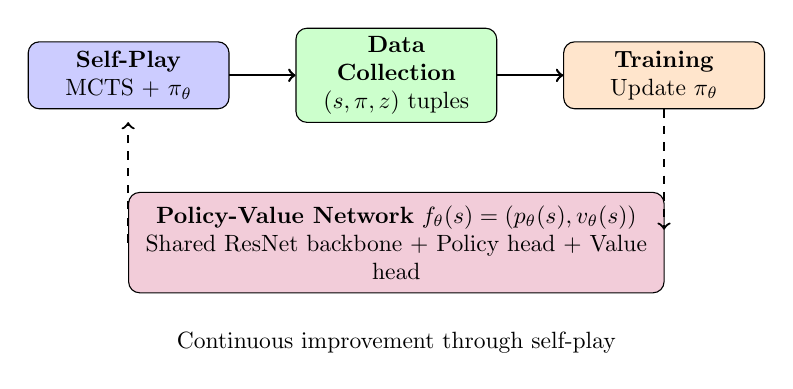
\begin{tikzpicture}[scale=0.85, transform shape]

    % Self-play loop
    \node[draw, rounded corners, fill=blue!20,
          minimum width=3.0cm, minimum height=1cm] (selfplay) at (2, 6) {
      \begin{minipage}{2.2cm}
        \centering
        \textbf{Self-Play} \\
        MCTS + $\pi_\theta$
      \end{minipage}
    };

    % Data collection
    \node[draw, rounded corners, fill=green!20,
          minimum width=3.0cm, minimum height=1cm] (datacollect) at (6, 6) {
      \begin{minipage}{2.2cm}
        \centering
        \textbf{Data Collection} \\
        $(s, \pi, z)$ tuples
      \end{minipage}
    };

    % Training
    \node[draw, rounded corners, fill=orange!20,
          minimum width=3.0cm, minimum height=1cm] (training) at (10, 6) {
      \begin{minipage}{2.2cm}
        \centering
        \textbf{Training} \\
        Update $\pi_\theta$
      \end{minipage}
    };

    % Neural network
    \node[draw, rounded corners, fill=purple!20,
          minimum width=8cm, minimum height=1.5cm] (network) at (6, 3.5) {
      \begin{minipage}{7.5cm}
        \centering
        \textbf{Policy-Value Network} $f_\theta(s) = (p_\theta(s), v_\theta(s))$ \\
        Shared ResNet backbone + Policy head + Value head
      \end{minipage}
    };

    % --------------------
    % Arrows
    % --------------------

    \draw[->, thick] (selfplay.east) -- (datacollect.west);
    \draw[->, thick] (datacollect.east) -- (training.west);


    \draw[->, thick] (selfplay.east) -- (datacollect.west);
    \draw[->, thick] (datacollect.east) -- (training.west);


    \draw[->, thick, dashed] (network.west) -- ++(0.0,1.8);

    \draw[->, thick, dashed] (training.south) -- ++(0.0,-1.8);

    \node[anchor=center] at (6, 2.0)
        {Continuous improvement through self-play};

  \end{tikzpicture}
  \end{center}

\end{frame}
% Slide 17: AlphaZero Training Objective
\begin{frame}{AlphaZero Training Objective}
  \begin{block}{Data Generation}
    Each self-play game generates training examples $(s_t, \pi_t, z)$ where:
    \begin{itemize}
      \item $s_t$: Game state at time $t$
      \item $\pi_t$: MCTS policy (visit count distribution)
      \item $z$: Game outcome from $s_t$'s player perspective
    \end{itemize}
  \end{block}
  
  \begin{block}{Loss Function}
    \[\mathcal{L}(\theta) = (z - v_\theta(s))^2 - \pi^T \log p_\theta(s) + c \|\theta\|_2^2\]
    where:
    \begin{itemize}
      \item Value loss: $(z - v_\theta(s))^2$ -- MSE between outcome and predicted value
      \item Policy loss: $-\pi^T \log p_\theta(s)$ -- Cross-entropy with MCTS policy
      \item Regularization: $c \|\theta\|_2^2$ -- L2 weight decay
    \end{itemize}
  \end{block}
  
\end{frame}

\begin{frame}{AlphaZero Self-Improvement Loop}
  \begin{alertblock}{Self-Improvement Loop}
    Better network $\rightarrow$ Better MCTS $\rightarrow$ Better training data $\rightarrow$ Better network
  \end{alertblock}

  \textbf{Implementation:} \texttt{exp06\_selfplay\_alphazero.py}
\end{frame}

% Slide 18: Implementation Architecture
\begin{frame}{Implementation Architecture Overview}
  \begin{block}{Core Components We'll Build}
    \begin{enumerate}
      \item \textbf{Gomoku 5×5 Environment}: Perfect information game for testing
      \item \textbf{Policy-Value Network}: CNN with dual heads
      \item \textbf{PUCT MCTS}: Tree search with neural guidance
      \item \textbf{Self-Play Trainer}: Data generation and model updates
      \item \textbf{Toy Language Model}: For DPO experiments
      \item \textbf{DPO Trainer}: Direct preference optimization
    \end{enumerate}
  \end{block}
  
\end{frame}

\begin{frame}{Implementation Architecture: Stacks}
  \begin{columns}[t]
    \begin{column}{0.48\textwidth}
      \textbf{Game Playing Stack}
      \begin{itemize}
        \item Gomoku environment
        \item ResNet policy-value network
        \item PUCT MCTS (25-100 simulations)
        \item Self-play training loop
        \item Tournament evaluation
      \end{itemize}
    \end{column}
    \begin{column}{0.48\textwidth}
      \textbf{Language Model Stack}
      \begin{itemize}
        \item Character-level tokenizer
        \item Small transformer (2-4 layers)
        \item Synthetic preference dataset
        \item DPO optimisation loop
        \item Preference accuracy metrics
      \end{itemize}
    \end{column}
  \end{columns}
\end{frame}

% Slide 19: Experimental Design Principles
\begin{frame}{Experimental Design Principles}
  \begin{block}{Reproducibility Requirements}
    \begin{itemize}
      \item Fixed random seeds (Python, NumPy, PyTorch)
      \item Deterministic CUDA operations where possible
      \item Version tracking (PyTorch, CUDA, library versions)
      \item Hardware specifications (CPU, GPU, memory)
      \item Hyperparameter logging and checkpointing
    \end{itemize}
  \end{block}
  
  \begin{block}{Performance Optimization}
    \begin{itemize}
      \item Mixed precision training (AMP) when available
      \item \texttt{torch.compile} for model acceleration
      \item Batched inference for MCTS tree expansion
      \item Efficient tensor operations and memory management
      \item CPU/GPU device handling and data transfer optimization
    \end{itemize}
  \end{block}
  
\end{frame}

\begin{frame}{Evaluation Metrics}
  \begin{itemize}
    \item \textbf{AlphaZero}: Win rate vs random, previous versions, search budget analysis
    \item \textbf{DPO}: Preference accuracy, KL divergence, perplexity changes
    \item \textbf{Both}: Training loss curves, convergence analysis, hyperparameter sensitivity
  \end{itemize}
\end{frame}



% Slide 21: Experiment 1 - Setup Verification
\begin{frame}{Experiment 1: Setup Verification}
  \textbf{Script:} \texttt{exp01\_setup\_verification.py}
  
  \begin{block}{Objectives}
    \begin{itemize}
      \item Verify PyTorch installation, device selection, and deterministic seeding
      \item Confirm Hugging Face tokenizer availability and simple Gomoku board checks
      \item Exercise AMP and \texttt{torch.compile} hooks needed for later experiments
    \end{itemize}
  \end{block}
  
  \begin{block}{Expected Output (seed 42)}
    \begin{itemize}
      \item Console prints device string (e.g., \texttt{cpu}) and PyTorch version
      \item Board diagnostic reports ``Legal actions: 23/25'' after placing two stones
      \item Mixed-precision test prints ``Mixed precision training: $\checkmark$'' when CUDA is available
    \end{itemize}
  \end{block}
  
\end{frame}

\begin{frame}[fragile]{Experiment 1: Setup Verification Code}
  \begin{lstlisting}
#!/usr/bin/env python3
"""Verify PyTorch, CUDA, transformers, and board diagnostics"""

import torch, random, numpy as np

def setup_seed(seed=42):
    random.seed(seed)
    np.random.seed(seed)
    torch.manual_seed(seed)
    if torch.cuda.is_available():
        torch.cuda.manual_seed_all(seed)

device = torch.device(
    "cuda" if torch.cuda.is_available()
    else "mps" if hasattr(torch.backends, "mps")
                    and torch.backends.mps.is_available()
    else "cpu"
)
setup_seed(42)

print(f"Device: {device}")
print(f"PyTorch version: {torch.__version__}")
print(f"CUDA available: {torch.cuda.is_available()}")
  \end{lstlisting}
\end{frame}

% Slide 22: Experiment 2 - Training Infrastructure
\begin{frame}{Experiment 2: Training Infrastructure}
  \textbf{Script:} \texttt{exp02\_standard\_training\_header.py}
  
  \begin{block}{Objectives}
    \begin{itemize}
      \item Provide reusable dataclass configs, checkpoint/save utilities, and logging scaffolding
      \item Exercise AMP-aware checkpoint saves that handle \texttt{torch.compile} wrapped modules
      \item Benchmark inference throughput and DQN updates with reproducible seeds
    \end{itemize}
  \end{block}
  
  \begin{block}{Expected Output (seed 42)}
    \begin{itemize}
      \item Console shows ``Config save/load: $\checkmark$'' followed by checkpoint save/load confirmations
      \item TensorBoard log directory created under \texttt{test\_logs/} with scalar entries
      \item Throughput line like ``Model throughput: 850.0 inferences/sec'' and a DQN loss scalar
    \end{itemize}
  \end{block}
  
\end{frame}

\begin{frame}[fragile]{Experiment 2: Config \& Checkpoint Code}
  \begin{lstlisting}
@dataclass
class ExperimentConfig:
    learning_rate: float = 1e-4
    batch_size: int = 32
    beta: float = 0.1          # DPO temperature
    c_puct: float = 1.0        # MCTS exploration
    num_simulations: int = 25  # MCTS budget
    device: str = str(device)
    seed: int = 42

class CheckpointManager:
    """Handles model checkpointing with torch.compile support"""

    def save_checkpoint(self, model, optimizer, epoch, metrics, config):
        model_state = (model.state_dict() if not hasattr(model, "_orig_mod")
                      else model._orig_mod.state_dict())

        checkpoint = {
            "model_state_dict": model_state,
            "optimizer_state_dict": optimizer.state_dict(),
            "epoch": epoch,
            "metrics": metrics,
            "config": asdict(config),
        }
        torch.save(checkpoint, checkpoint_path)
  \end{lstlisting}
\end{frame}

% Slide 23: Experiment 3 - Gomoku Environment
\begin{frame}{Experiment 3: Gomoku 5×5 Environment}
  \textbf{Script:} \texttt{exp03\_gomoku\_environment.py}
  
  \begin{block}{Objectives}
    \begin{itemize}
      \item Implement a 5×5 Gomoku environment with legal action masks and terminal detection
      \item Validate perspective switching, cloning, and horizontal/diagonal win checks
      \item Produce board summaries for downstream MCTS/AlphaZero experiments
    \end{itemize}
  \end{block}
  
  \begin{block}{Expected Output (seed 42)}
    \begin{itemize}
      \item Sequence of ``Testing …'' lines concluding with ``All tests passed! $\checkmark$''
      \item Demonstration game trace printing moves and rewards, finishing with detected winner
      \item Environment specification footer confirming board size, action count, and observation shape
    \end{itemize}
  \end{block}
  
\end{frame}

\begin{frame}[fragile]{Experiment 3: Gomoku Environment Snippet}
  \begin{lstlisting}
class Gomoku5x5:
    """5x5 Gomoku with perspective-based observations"""

    def reset(self):
        self.board = np.zeros((5, 5), dtype=np.int8)
        self.current_player = 1  # Black starts
        return self._get_observation(), {}

    def _get_observation(self):
        current_stones = (self.board == self.current_player)
        opponent_stones = (self.board == -self.current_player)
        obs = np.stack([current_stones, opponent_stones], axis=0)
        return torch.from_numpy(obs.astype(np.float32))

    def step(self, action):
        row, col = divmod(action, 5)
        self.board[row, col] = self.current_player

        winner = self._check_winner()
        if winner != 0:
            reward = 1.0 if winner == self.current_player else -1.0
            return self._get_observation(), reward, True, False, {}

        self.current_player *= -1
        return self._get_observation(), 0.0, False, False, {}
  \end{lstlisting}
\end{frame}

% Slide 24: Experiment 4 - Policy-Value Network
\begin{frame}{Experiment 4: Policy-Value Network}
  \textbf{Script:} \texttt{exp04\_policy\_value\_network.py}
  
  \begin{block}{Objectives}
    \begin{itemize}
      \item Build a shared-convolution trunk with dual policy/value heads for Gomoku boards
      \item Support legal action masking, AMP-aware forward passes, and optional \texttt{torch.compile}
      \item Provide a trainer utility for supervised policy/value updates from self-play data
    \end{itemize}
  \end{block}
  
  \begin{block}{Expected Output (seed 42)}
    \begin{itemize}
      \item Reports total parameter count ($\approx$1.1M) and marks ``Architecture: $\checkmark$''
      \item Training step summary with scalar losses and ``Evaluation: $\checkmark$'' once metrics computed
      \item Demo section prints value estimate ($\approx$0.0 at reset) and top-5 move probabilities
    \end{itemize}
  \end{block}
  
\end{frame}

\begin{frame}[fragile]{Experiment 4: Policy-Value Network Snippet}
  \begin{lstlisting}
class PolicyValueNet(nn.Module):
    """ResNet-style CNN with policy and value heads"""

    def __init__(self, input_channels=2, hidden_channels=64,
                 num_residual_blocks=4):
        super().__init__()
        self.stem = nn.Sequential(
            nn.Conv2d(input_channels, hidden_channels, 3, padding=1),
            nn.BatchNorm2d(hidden_channels), nn.ReLU(),
        )
        self.residual_blocks = nn.ModuleList(
            ResidualBlock(hidden_channels) for _ in range(num_residual_blocks)
        )
        self.policy_head = nn.Sequential(
            nn.Conv2d(hidden_channels, 2, 1), nn.BatchNorm2d(2),
            nn.ReLU(), nn.Flatten(), nn.Linear(50, 25),
        )
        self.value_head = nn.Sequential(
            nn.Conv2d(hidden_channels, 1, 1), nn.BatchNorm2d(1),
            nn.ReLU(), nn.Flatten(), nn.Linear(25, 64),
            nn.ReLU(), nn.Linear(64, 1), nn.Tanh(),
        )
  \end{lstlisting}
\end{frame}

% Slide 25: Experiment 5 - PUCT MCTS
\begin{frame}{Experiment 5: PUCT MCTS Implementation}
  \textbf{Script:} \texttt{exp05\_puct\_mcts.py}
  
  \begin{block}{Objectives}
    \begin{itemize}
      \item Implement PUCT selection with visit counts, priors, and mean value updates
      \item Support batched neural guidance by coupling to the policy-value net
      \item Provide temperature control, Dirichlet noise, and performance benchmarks
    \end{itemize}
  \end{block}
  
  \begin{block}{Expected Output (seed 42)}
    \begin{itemize}
      \item ``Testing MCTS node: $\checkmark$'' followed by ``MCTS search: $\checkmark$'' when Gomoku + network available
      \item Benchmark lines such as ``25 simulations: 0.087s per search'' (CPU numbers slightly higher)
      \item Demo trace listing moves with root values and top-3 action probabilities until termination
    \end{itemize}
  \end{block}
  
\end{frame}

\begin{frame}[fragile]{Experiment 5: MCTS Node Snippet}
  \begin{lstlisting}
class MCTSNode:
    def __init__(self, prior=0.0, parent=None):
        self.parent = parent
        self.children = {}
        self.N, self.W, self.Q = 0, 0.0, 0.0
        self.P = prior

    def select_action(self, c_puct):
        def puct_value(action, child):
            if child.N == 0:
                return float('inf')
            bonus = c_puct * child.P * math.sqrt(self.N) / (1 + child.N)
            return child.Q + bonus
        return max(self.children, key=lambda a: puct_value(a, self.children[a]))

    def backup(self, value):
        self.N += 1
        self.W += value
        self.Q = self.W / self.N
        if self.parent:
            self.parent.backup(-value)
  \end{lstlisting}
\end{frame}

% Slide 26: Experiment 6 - AlphaZero Self-Play
\begin{frame}{Experiment 6: AlphaZero Self-Play Training}
  \textbf{Script:} \texttt{exp06\_selfplay\_alphazero.py}
  
  \begin{block}{Objectives}
    \begin{itemize}
      \item Combine MCTS policy targets with replay buffer for AlphaZero-style updates
      \item Track self-play outcomes, buffer growth, and supervised training loss
      \item Provide evaluation hooks against random opponents for quick smoke tests
    \end{itemize}
  \end{block}
  
  \begin{block}{Expected Output (seed 42)}
    \begin{itemize}
      \item ``Experience buffer: $\checkmark$'' and ``Self-play trainer: $\checkmark$'' when MCTS is available
      \item Demo logs summarizing games (e.g., ``Game 2: Black wins in 17 moves'') and buffer size
      \item Evaluation block with win/draw/loss rates (random baseline $\approx$33% each before training)
    \end{itemize}
  \end{block}
  
\end{frame}

\begin{frame}[fragile]{Experiment 6: Self-Play Loop Snippet}
  \begin{lstlisting}
class SelfPlayTrainer:
    def play_game(self, env):
        """Collect one self-play game and return training triples."""
        trajectories = []
        env.reset()
        while not env.is_terminal():
            temp = 1.0 if len(trajectories) < 10 else 0.0
            action_probs, _ = self.mcts.search(env, 25, temp)
            policy = torch.zeros(25)
            for action, prob in action_probs.items():
                policy[action] = prob
            trajectories.append((env._get_observation().clone(), policy, env.current_player))
            action = np.random.choice(list(action_probs), p=list(action_probs.values()))
            env.step(action)

        winner = env.winner()
        def target(player):
            return 1.0 if winner == player else -1.0 if winner else 0.0
        return [Experience(state, policy, target(player))
                for state, policy, player in trajectories]
  \end{lstlisting}
\end{frame}

% Slide 27: Experiment 7 - Toy Language Model
\begin{frame}{Experiment 7: Toy Language Model for DPO}
  \textbf{Script:} \texttt{exp07\_toy\_causal\_lm.py}
  
  \begin{block}{Objectives}
    \begin{itemize}
      \item Build a lightweight tokenizer and causal transformer compatible with DPO training
      \item Generate a synthetic preference dataset with (prompt, chosen, rejected) triples
      \item Provide sampling helpers for quick qualitative evaluation of generated text
    \end{itemize}
  \end{block}
  
  \begin{block}{Expected Output (seed 42)}
    \begin{itemize}
      \item ``Tokenizer: $\checkmark$'' with reported vocab size (default 512) and model parameter count
      \item Sample generation snippet showing prompt/completion pairs from the tiny model
      \item Preference dataset preview printing tokenized chosen vs rejected responses
    \end{itemize}
  \end{block}
  
\end{frame}

\begin{frame}[fragile]{Experiment 7: Tokenizer \& LM Snippet}
  \begin{lstlisting}
class SimpleTokenizer:
    def __init__(self, vocab_size=512):
        chars = string.ascii_letters + string.digits + string.punctuation + " "
        specials = ["<PAD>", "<BOS>", "<EOS>", "<UNK>"]
        vocab_chars = list(set(chars))[:vocab_size - len(specials)]
        self.vocab = specials + vocab_chars
        self.token_to_id = {token: i for i, token in enumerate(self.vocab)}

class SimpleTransformerLM(nn.Module):
    def __init__(self, vocab_size, embed_dim=128, num_layers=2):
        super().__init__()
        self.token_embedding = nn.Embedding(vocab_size, embed_dim)
        self.position_embedding = nn.Embedding(128, embed_dim)
        self.layers = nn.ModuleList(
            TransformerBlock(embed_dim, num_heads=4) for _ in range(num_layers)
        )
        self.lm_head = nn.Linear(embed_dim, vocab_size, bias=False)
  \end{lstlisting}
\end{frame}

% Slide 28: Experiment 8 - DPO Implementation
\begin{frame}{Experiment 8: DPO Loss and Training}
  \textbf{Script:} \texttt{exp08\_dpo\_implementation.py}
  
  \begin{block}{Objectives}
    \begin{itemize}
      \item Implement DPO loss with implicit KL regularisation against a frozen reference model
      \item Support mixed-precision training loops and dataset iteration over preference batches
      \item Track accuracy, reward margins, and KL drift for post-lecture analysis
    \end{itemize}
  \end{block}
  
  \begin{block}{Expected Output (seed 42)}
    \begin{itemize}
      \item ``Testing DPO loss…'' followed by ``DPO loss computation: $\checkmark$'' and ``Training step: $\checkmark$''
      \item Demo run logging training/validation losses ($\approx$0.69 → 0.55) and accuracy improving >60%
      \item Beta sweep summary such as ``Beta 0.1: Accuracy = 0.62, KL = 0.08'' for sensitivity checks
    \end{itemize}
  \end{block}
  
\end{frame}

\begin{frame}[fragile]{Experiment 8: DPO Loss Snippet}
  \begin{lstlisting}
def dpo_loss(policy_chosen_logps, policy_rejected_logps,
             reference_chosen_logps, reference_rejected_logps, beta):
    policy_diff = policy_chosen_logps - policy_rejected_logps
    reference_diff = reference_chosen_logps - reference_rejected_logps

    logits = beta * (policy_diff - reference_diff)
    loss = -F.logsigmoid(logits).mean()
    accuracy = (logits > 0).float().mean()

    reward_margin = beta * ((policy_chosen_logps - reference_chosen_logps)
                            - (policy_rejected_logps - reference_rejected_logps))
    return {
        "loss": loss,
        "accuracy": accuracy,
        "reward_margin": reward_margin.mean(),
    }
  \end{lstlisting}
\end{frame}

\begin{frame}[fragile]{Experiment 8: Mixed Precision Step}
  \begin{lstlisting}
with torch.autocast(device_type="cuda" if amp_enabled else "cpu"):
    policy_chosen = compute_log_likelihood(policy_model, chosen_ids, chosen_mask)
    policy_rejected = compute_log_likelihood(policy_model, rejected_ids, rejected_mask)
    with torch.no_grad():
        ref_chosen = compute_log_likelihood(ref_model, chosen_ids, chosen_mask)
        ref_rejected = compute_log_likelihood(ref_model, rejected_ids, rejected_mask)
    loss_dict = dpo_loss(policy_chosen, policy_rejected, ref_chosen, ref_rejected, beta)
  \end{lstlisting}
\end{frame}

% Slide 29: Experiment 9 - Integration Testing
\begin{frame}{Experiment 9: Integration Testing \& Benchmarks}
  \textbf{Script:} \texttt{exp09\_integrated\_capstone\_test.py}
  
  \begin{block}{Comprehensive Test Suite}
    \begin{itemize}
      \item \textbf{Component Tests}: Individual module functionality
      \item \textbf{Integration Tests}: End-to-end pipeline validation
      \item \textbf{Reproducibility Tests}: Fixed seed consistency
      \item \textbf{Performance Benchmarks}: Throughput and timing measurements
    \end{itemize}
  \end{block}
  
  \begin{block}{Expected Output (seed 42)}
    \begin{itemize}
      \item Console banner ``LECTURE 11 INTEGRATION TEST SUITE'' followed by eight PASS entries
      \item Summary line ``Success Rate: 9/9 tests passed'' (CPU runs may skip performance timings gracefully)
      \item JSON report saved to \texttt{runs/integration\_suite/integration\_report.json}
    \end{itemize}
  \end{block}
  
\end{frame}


\begin{frame}[fragile]{Experiment 9: Runner Skeleton}
  \begin{lstlisting}
from lecture11.experiments import EXPERIMENT_ROOT, RUNS_ROOT

class IntegrationTestSuite:
    def __init__(self):
        self.test_results: dict[str, dict[str, object]] = {}
        self.artifacts_dir = (RUNS_ROOT / "integration_suite")
        self.artifacts_dir.mkdir(parents=True, exist_ok=True)
        self.configs_dir = self.artifacts_dir / "configs"
        self.checkpoints_dir = self.artifacts_dir / "checkpoints"
        for folder in (self.configs_dir, self.checkpoints_dir):
            folder.mkdir(parents=True, exist_ok=True)

    def run_all_tests(self) -> dict[str, object]:
        print("=" * 60)
        print("LECTURE 11 INTEGRATION TEST SUITE")
        self.test_results["environment"] = self.test_environment_setup()
        self.test_results["integration"] = self.test_full_integration()
        return self.generate_test_report()
\end{lstlisting}
\end{frame}

% Slide 30: Key Implementation Insights (AlphaZero)
\begin{frame}{Key Implementation Insights: AlphaZero}
  \begin{itemize}
    \item Temperature annealing: high early temperature, greedy late in games.
    \item Dirichlet noise only at the root to encourage exploration.
    \item Perspective handling: always view the board from the current player.
    \item Experience replay via reservoir sampling for diverse batches.
    \item Evaluate against previous checkpoints and random baselines.
  \end{itemize}
\end{frame}

% Slide 30b: Key Implementation Insights (DPO)
\begin{frame}{Key Implementation Insights: DPO}
  \begin{itemize}
    \item Keep the reference model frozen to avoid distribution shift.
    \item Tune $\beta$: larger values emphasise preference margins but weaken KL penalties.
    \item Sum sequence-level log-probs with proper padding masks.
    \item Log-sigmoid retains numerical stability during optimisation.
    \item Track preference accuracy and implicit KL divergence each epoch.
  \end{itemize}

  \begin{alertblock}{Common Pitfalls}
    Masking bugs, missing regularisation, or device placement errors quickly destabilise training.
  \end{alertblock}
\end{frame}

% Slide 31: Hyperparameter Sensitivity (AlphaZero)
\begin{frame}{Hyperparameter Sensitivity: AlphaZero}
  \begin{itemize}
    \item $c_{\text{puct}}$: explore strength (0.5–2.0).
    \item Number of simulations: 10–100 per move.
    \item Temperature decay: when to switch to greedy play.
    \item Dirichlet $\alpha$: controls exploration noise at the root.
    \item Optimiser settings: learning rate, weight decay, gradient clipping.
  \end{itemize}
\end{frame}

% Slide 31b: Hyperparameter Sensitivity (DPO)
\begin{frame}{Hyperparameter Sensitivity: DPO}
  \begin{itemize}
    \item $\beta$ in [0.01, 1.0] sets preference strength.
    \item Learning rate typically lower than SFT baselines.
    \item Batch size and sequence length tied to GPU memory.
    \item Warmup steps and scheduler smoothing for stable optimisation.
  \end{itemize}

  \begin{block}{Experimental Design Tips}
    \begin{itemize}
      \item Grid or random search across the most sensitive knobs.
      \item Multiple random seeds for statistically meaningful comparisons.
      \item Inspect learning curves and ablations to isolate components.
    \end{itemize}
  \end{block}
\end{frame}

% Slide 32: Scaling to Real Applications (Engineering)
\begin{frame}{Scaling to Real Applications: Engineering}
  \begin{block}{Computational Scaling}
    \begin{itemize}
      \item Distributed MCTS and parallel rollouts.
      \item Model or tensor parallelism for larger networks.
      \item Gradient accumulation for big batches.
      \item Mixed precision training for throughput.
      \item Efficient data loading and preprocessing pipelines.
    \end{itemize}
  \end{block}

  \begin{block}{Methodological Extensions}
    \begin{itemize}
      \item Curriculum or multi-task learning for complex domains.
      \item Transfer learning and continual adaptation.
      \item Human-in-the-loop refinement and evaluation.
    \end{itemize}
  \end{block}
\end{frame}

% Slide 32b: Scaling to Real Applications (Use Cases)
\begin{frame}{Scaling to Real Applications: Use Cases}
  \begin{itemize}
    \item Game playing: Chess, Go, StarCraft, Poker.
    \item Language models: RLHF/DPO for chat assistants.
    \item Robotics: Manipulation, navigation, dexterous control.
    \item Science: Protein folding, drug discovery, theorem proving.
    \item Finance: Trading strategies, risk management, portfolio optimisation.
  \end{itemize}
\end{frame}

% Slide 33: Research Frontiers (RLHF/DPO)
\begin{frame}{Research Frontiers: RLHF \& DPO}
  \begin{itemize}
    \item Constitutional AI and multi-layered preference learning.
    \item RLAIF: AI-generated feedback to scale supervision.
    \item Iterative DPO pipelines with refreshed preference data.
    \item Multi-objective optimisation balancing safety, helpfulness, style.
    \item Modelling preference uncertainty and annotator disagreement.
  \end{itemize}
\end{frame}

% Slide 33b: Research Frontiers (Planning)
\begin{frame}{Research Frontiers: Planning}
  \begin{itemize}
    \item MuZero-style learned dynamics for model-based planning.
    \item Gumbel AlphaZero and improved sampling strategies.
    \item Continuous-action and partial-observability extensions to MCTS.
    \item Multi-agent search algorithms for competitive settings.
  \end{itemize}

  \begin{alertblock}{Emerging Trends}
    Foundation models with RLHF/DPO, multi-modal preference learning, and scalable oversight methods.
  \end{alertblock}
\end{frame}



% Slide 39: Key Takeaways (Technical)
\begin{frame}{Key Takeaways: Technical}
  \begin{itemize}
    \item RLHF/DPO removes the reward model by optimising preferences directly.
    \item Neural-guided MCTS powers AlphaZero-style planning loops.
    \item Self-improvement requires careful data pipelines and evaluation.
    \item Implementation details (logging, seeding, hardware) matter for reproducibility.
  \end{itemize}
\end{frame}

% Slide 39b: Key Takeaways (Perspective)
\begin{frame}{Key Takeaways: Perspective}
  \begin{itemize}
    \item Modern RL blends search, learning, and preferences in one system.
    \item Rigorous evaluation means multiple metrics and statistical tests.
    \item Grow complexity gradually: validate components before scaling.
    \item Ethics and safety considerations are integral to deployment.
  \end{itemize}
\end{frame}


\end{document}
